\documentclass[]{article}
\usepackage[margin=1.5in]{geometry}
\usepackage{setspace}
\usepackage{graphicx}
\usepackage{hyperref}
\usepackage{array}

\onehalfspacing
%opening
\title{ParkMe: Software Requirements Specification}
\author{Daniel Agostinho\\agostd - 001414323\\ Group 5 \and Michael Bitzos\\bitzosm - 001405050\\ Group 5 \and Kathryn Brownlee\\brownlks - 001408416\\ Group 5  \and Anthony Chang\\changa7 - 001413615\\ Group 5 \and Ben Petkovsek\\petkovb - 001417104\\ Group 5}


\begin{document}
\date{November 4, 2018}
\maketitle
\newpage
\tableofcontents
\newpage

\section{Introduction}
At one point or another everyone who drives has encountered this scenario; you plan to go to a mall for the day so you drive all the way there only to discover that the parking lot is seemingly full. You must frustratingly drive around the parking area to try and find a single spot, if you even find one. This problem has existed for as long as vehicles have, and while some rudimentary and limited solutions exist such as a parking structure noting how many open spots exist when you enter, there are no solutions that an average consumer can use to solve the problem preemptively. Imagine if there was a way that you could know exactly how many spots were open in a parking lot at a given time and where they were, before you even left your house. 

On the other hand, imagine being a business owner and having the ability to see trends in how many visitors arrived on a given day, how long the average visitor stayed, or even if a vehicle has been parked in a paid spot for longer than they should. ParkMe is a mobile application and parking availability system that aims to provide valuable information not only to customers, but also businesses.


\subsection{Behaviour Overview}
To solve the problems mentioned above, ParkMe will implement several general systems. The first and most important of these is the ability to monitor the occupancy of parking spots in a given parking area through a series of physical sensors. This data will then be used by the mobile application to update the customer on the number of available spots in the lot, as well as the location of those spots. Specific data on information such as accessible parking, expectant mothers, paid parking...etc will also be displayed, and will utilize preferences set by the user. 

Ideally, the application will also include functionality to navigate the user to a parking spot/row/area, but this integration will depend on the accuracy and availability of GPS systems and the complexity of those systems. In addition, a secondary section of the application which will only be available to verified business owners will include various statistics and trends based on the data gathered by the system, allowing those owners to better tailor their experience to the customers, and increasing returns as well.



\subsection{Scope}
ParkMe will allow customer users to receive up-to-date information on the availability of parking spots in a desired lot. They will be able to know where their desired parking spot is, and may also be able to get navigation to the spot. Additionally, they will be able to mark where they parked.  The business users will be able to access a separate interface where they can view information and statistics that can be made from the parking data. These may include things such as average occupancy rates for parking spots, overall number of visits and departures based on time/day...etc.

\subsubsection{Stakeholders}
There are two main stakeholders who will be interested in our product, the consumers, and businesses. The consumers are the everyday people who use the application for parking availability. The businesses can constitute two groups, but are handled in the same way. One of these groups is the small business, who owns a smaller lot and is interested in customer information and trends. The second group is the large business. This group is composed of entities such as the owner of an entire mall, rather than the individual businesses inside of the mall who wouldn’t be able to glean any useful information from the parking trends. Making sure that both of these groups find our system useful is imperative for its success.

The consumer will find use in knowing that parking spots are open for a store they wish to visit, and will have less frustration physically finding a spot. This is good for both the consumer and the business, as it will ensure that not being able to find a parking spot will not deter a potential customer.The business will find use in being able to recognize trends in their customer attendance, allowing them to make changes which improve their own potential goals as well as improving the experience for the customer. In this way, ParkMe satisfies both major stakeholders and the relationship between them is strengthened as well.

\section{Constants}

\begin{itemize}
	\item PARKING\_SPOT\_RESPONSE\_TIME= 500ms 
	\begin{itemize}
		\item How long it takes for the availability of a parking spot to update on the application.
	\end{itemize}

	\item PARKING\_SPOT\_EXPIRATION\_TIME\_WARNING= 10 minutes
	\begin{itemize}
		\item How long before the application will notify the user their parking spot is about to expire.
	\end{itemize}

	\item MAX\_ANALYTICS\_DATA= 50gb
	\begin{itemize}
		\item How much analytics data will be recorded before older data will be deleted.
	\end{itemize}

	\item MAX\_CONCURRENT\_USERS= 1000 users
	\begin{itemize}
		\item How many concurrent users our system will support.
	\end{itemize}

	\item DETECTION\_ERROR\_RATE= 0.01%
	\begin{itemize}
		\item Max errors in detection in percentage the system should maintain before.
	\end{itemize}
\end{itemize}
\section{Context Diagrams}

\graphicspath{ {./images/} }
	\begin{center}
		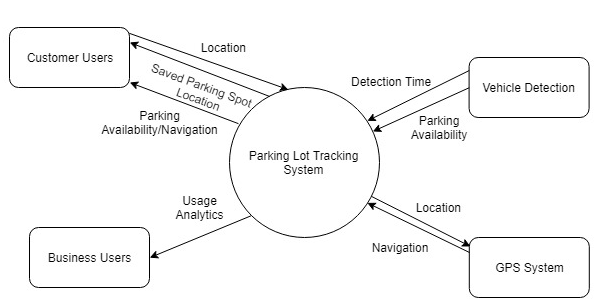
\includegraphics{context-diagram}
		\textbf{Figure 1: Context Diagram showing data flow of the system.}
	\end{center}

\section{Monitored and Controlled Variables}
ParkMe only contains two systems where it interacts with the environment around it: The mobile application where the user interacts with our system directly and the system responds back. The parking identifier is the second system where the users only interact with it and it does not directly interact with it.


\begin{table}
	\subsection{Monitored Variables}
	\begin{tabular}{ | m{3.5cm} | m{2cm}| m{2cm}| m{3cm}| m{3cm} |} 
		\hline
		Name & Type & Range & Units & Physical Interpretation \\ [0.5ex] 
		\hline
		Vehicle\_Detection & Status & "yes"/"no" & Unitless & If the Parking Spot Identifier has detected a vehicle or obstacle in the way. \\ 
		\hline
		Vehicle\_Detection\_Time & Number & [0, 31536000] & Seconds & The amount of time that has passed since an object has been detected by the sensor. \\
		\hline
		User\_GPS\_Data & GPS & Longitude: -180 ,180
		Latitude: -90, 90
	 & Longitude, Latitude in Degrees & The GPS location data of the users mobile device. \\ 
		\hline 
		User\_Device\_Rotation & Vector2 (Number, Number) & Does not have a range & Unitless & The rotation of the mobile device relative to the normal of the device. \\
		\hline
		User\_Application\_Input & Action & Does not have a range & Unitless & The user’s varied input to the mobile application** \\	
		\hline
	\end{tabular}\textbf{\caption{Monitored Variables for ParkMe}}
** - User inputs will be later described in the requirements section, this is just the general idea of inputs being registered from the environment from the user that all falls under potential application actions.
\end{table}

\begin{table}
	\subsection{Controlled Variables}
	\begin{tabular}{ | m{3.5cm} | m{2cm}| m{2cm}| m{3cm}| m{3cm} |} 
		\hline
		Name & Type & Range & Units & Physical Interpretation \\ [0.5ex] 
		\hline
		User\_Navigation & -- & -- & -- & The navigation the application uses to guide the user to the parking lot. \\ 
		\hline
		Parking\_Spot\_Availability & Status & On/Off & Unitless & If the parking  spot is occupied. \\
		\hline
		Parking\_Lot\_Statuses & List of Statuses & List of On/Off & Unitless & A mapping of the parking lot that the user requested with their availabilities. \\ 
		\hline 
		Parking\_Lot\_Analytics & Numbers & Varied & Varied & The statistics and trends relating to a parking lot/parking spot.** \\	
		\hline
	\end{tabular}\textbf{\caption{Controlled Variables for ParkMe}}
	** - User inputs will be later described in the requirements section, this is just the general idea of inputs being registered from the environment from the user that all falls under potential application actions.
\end{table}



\section{Functional Decomposition Diagram}
\begin{center}
	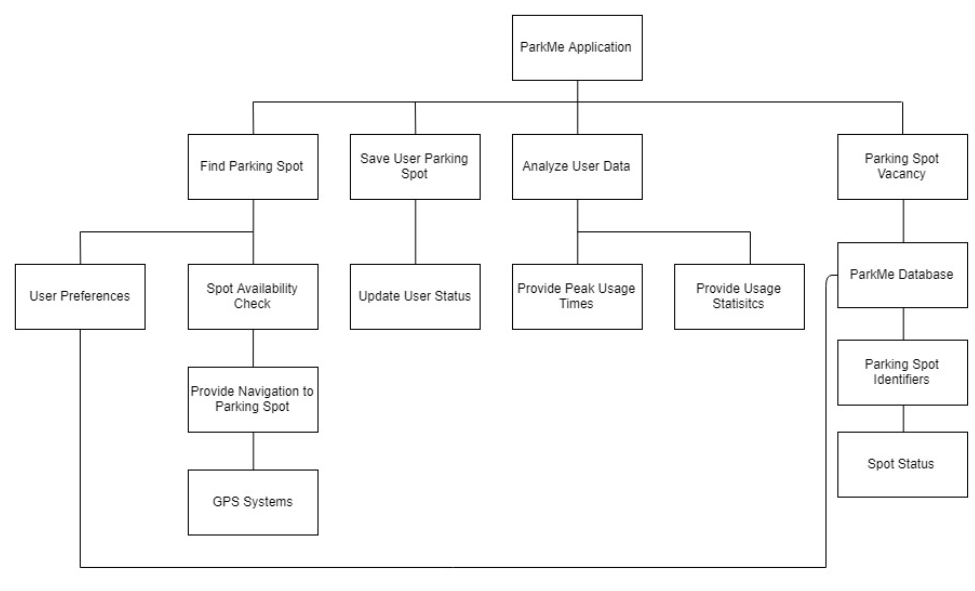
\includegraphics[width=\textwidth,height=\textheight,keepaspectratio]{fdd}
	\textbf{Figure 2: Functional Decomposition}
\end{center}

\section{Use Case Diagrams}
\begin{center}
	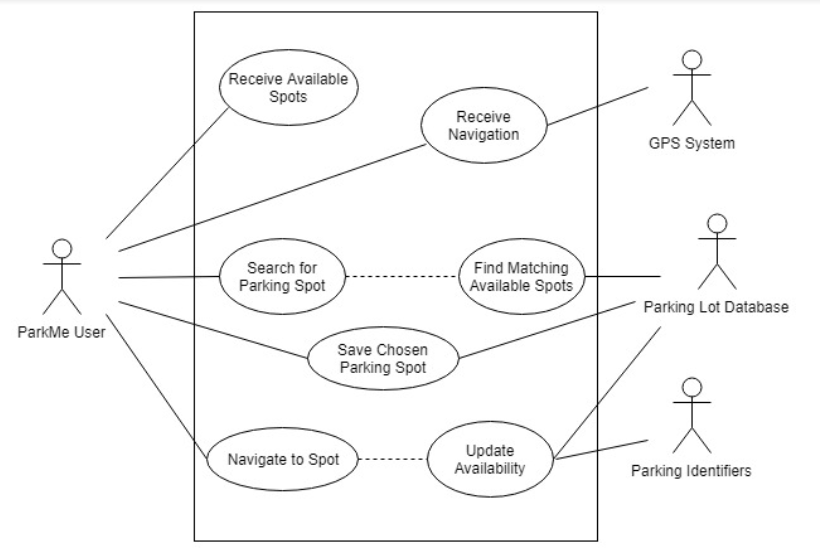
\includegraphics[width=\textwidth,height=\textheight,keepaspectratio]{uc1}
	\textbf{Figure 3: Use Case diagram for a driver using the app to find and navigate to an available parking spot.}
\end{center}
\begin{center}
	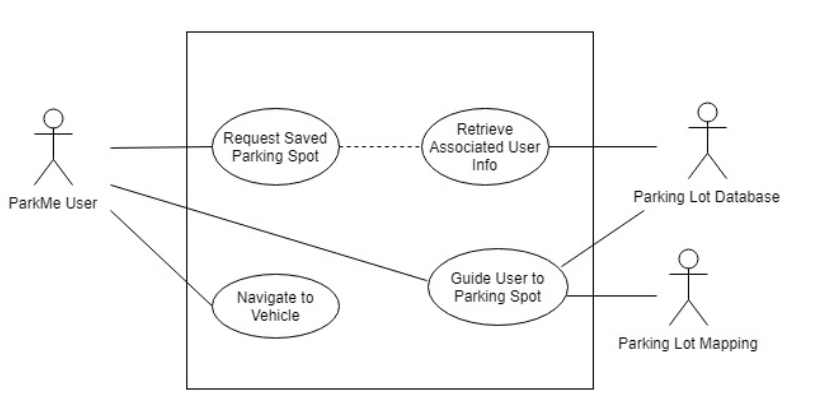
\includegraphics[width=\textwidth,height=\textheight,keepaspectratio]{uc2}
	\textbf{Figure 4: Use Case diagram for a customer returning to their vehicle using the saved parking spot location.}
\end{center}
\begin{center}
	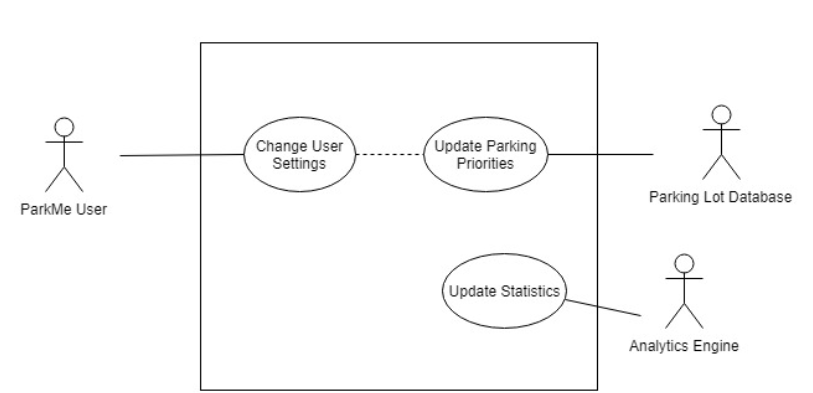
\includegraphics[width=\textwidth,height=\textheight,keepaspectratio]{uc3}
	\textbf{Figure 5: Use Case diagram for a user’s personalized settings being changed. This affects the user’s computed spot suggestion based on given choices and accessibility info.}
\end{center}
\begin{center}
	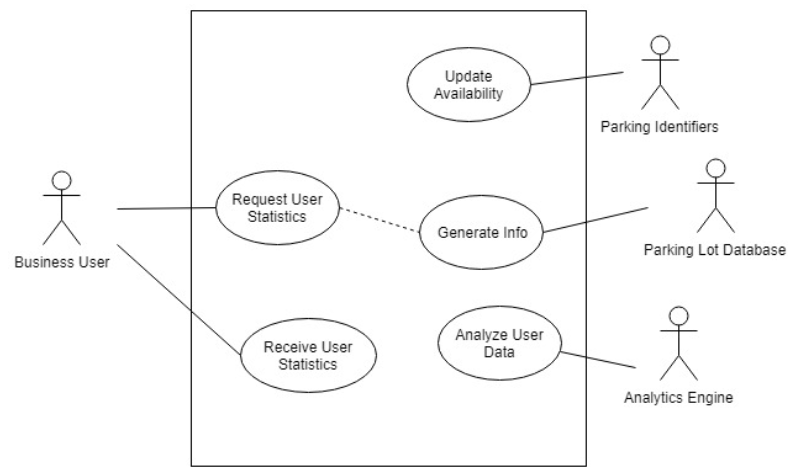
\includegraphics[width=\textwidth,height=\textheight,keepaspectratio]{uc4}
	\textbf{Figure 6: Use Case diagram for Business Users requesting user and parking lot statistics.}
\end{center}
	

\section{Requirements}
For the following requirements, let LC denote the requirements that are likely to change and UC denote the requirements that are unlikely to change.
\subsection{Functional Requirements}
	\subsubsection{Parking Detection Requirements}
	\begin{itemize}
		\item PDR1: The system must be able to recognize the state of vacancy of all parking spots in a parking lot. 
		\item PDR2:  The system must update the application with the status of parking spaces.
	\end{itemize}

	\subsubsection{Application Requirements}
	\begin{itemize}
		\item APR1: The system must provide the user with the number of available parking spots in a parking lot.
		
		\item APR2: [LC] The system should show a view of all available parking lots supported by ParkMe.
		\begin{itemize}
			\item This requirement might not be included in future revisions. 
		\end{itemize}
		
		\item APR3: The system must allow the user to select a parking lot that is supported by ParkMe.
	
		\item APR4: [LC] The system must provide navigation to the parking lot selected.
		\begin{itemize}
			\item This requirement might not be included in future revisions.
		\end{itemize}
		
		\item APR5: The system must keep track of the location where the user parked their vehicle in the parking lot.
		
		\item APR6: The users will be able to save what parking spot they parked in.
		
		\item APR7: The system must show if the parking spot is an accessibility parking only.
		
		\item APR8: The system must not show any vacant accessibility parking spots as available if the user has not specified accessible parking.
		
		\item APR9: [LC] The system must show if there is a time limit associated with a parking space.
		\begin{itemize}
			\item This requirement might not be included in future revisions.
		\end{itemize}
	
		\item APR10: [LC] The user must be warned if their time limited parking space will expire in PARKING\_SPACE\_EXPIRATION\_TIME\_WARNING.
		\begin{itemize}
			\item This requirement is dependent on if APR9 still holds.
		\end{itemize}
		
		\item APR11: [LC] When the user is navigating to the parking lot, the system must update the user’s position on the map and provide navigation instructions.
		\begin{itemize}
			\item This requirement is dependent on if APR4 still holds.
		\end{itemize}
		
		\item APR12: The system must notify the user when the parking lot does not have any vacant spots.
		
		\item APR13: [LC] The system must show the distance to the closest building entrance from the user’s selected parking space.
		\begin{itemize}
			\item This requirement is dependent on whether during development, access to entrance information is provided.
		\end{itemize}
		
		
		\item APR14: [UC] The application will warn the user to be cautious during the hours of 8pm and 8am and/or when parking lots are less than 10 percent occupied. (The purpose of this is to remind users to be safe at night where parking lots/garages can be unsafe.)
		\begin{itemize}
			\item While simple to implement it is an additional non-critical feature that may extend development time.
		\end{itemize}
	\end{itemize}
\subsubsection{Analytics Requirements}
\begin{itemize}
	\item ANR1: The application will show the user’s statistical averages of the vacancy of the parking lot. 
	\item ANR2: The application will show the user peak traffic times for each parking lot.
\end{itemize}

\subsubsection{Business User Requirements}
\begin{itemize}
	\item BUR1: [LC] The application must notify the business owner when a vehicle has been parked in a spot for longer than allowed.
	\begin{itemize}
		\item This requirement depends on the information given to the system by the business.
	\end{itemize}
	\item BUR2:  The application should provide the business users with information on each specific parking space by location and type.
	\item BUR3: The application should provide business users with trends about the parking lot.
	\item BUR4: [LC] The system will record up to MAX\_ANALYTICS\_DATA worth of analytics data while it is online.
	\begin{itemize}
		\item The amount of data that will be used could easily change based on other requirements
	\end{itemize}
\end{itemize}

	
	

	
\subsection{Nonfunctional Requirements}
\subsubsection{Look and Feel Requirements}
\begin{itemize}
	\item LF1: The applications user interface will adjust with device’s screen size specifications.
\end{itemize}
\subsubsection{Usability Requirements}
\begin{itemize}
	\item UR1: The mobile application should be easy to use and understand. Users should be able to perform basic functionality without addition instructions.
	\begin{itemize}
		\item Interface should be simple with high discoverability.
	\end{itemize}
	\item UR2: Interface will follow standard conventions (buttons, hamburger menu, etc.) and constraints will prevent users from performing undesired actions.
	\begin{itemize}
		\item The user interface should be familiar to the user and mappings should be intuitive to minimize learning time and mistakes.
		\item Constraints can help limit the possible actions a user can take and prevent some errors from occurring.
	\end{itemize}
	\item UR3: The application will provide sufficient error messages on error occurrences.
\end{itemize}

\subsubsection{Performance Requirements}
\begin{itemize}
	\item PR1: [LC] Users should be able to use the mobile application with low response time. Any communication done between client and server should be completed within PARKING\_SPACE\_RESPONSE\_TIME.
	\begin{itemize}
		\item The application need to receive a response and update to provide accurate information (parking spot is actually available and was not taken).
		\item This is likely to change as PARKING\_SPACE\_RESPONSE\_TIME is likely to change.
	\end{itemize}

	\item PR2: [LC] Servers should be able to sustain MAX\_CONCURRENT\_USERS.
	\begin{itemize}
		\item Depending on parking lot sizes and if a single server will host multiple parking lots, it needs to be able to receive and respond to requests without delay
		\item The supported amount of concurrent users can change with increased budget and better server capabilities
	\end{itemize}

	\item UR3: [LC] Parking space availability detection should have a error rare less than DETECTION\_ERROR\_RATE
	\begin{itemize}
		\item inimal false positives (reading a spot is occupied when it’s not or vice versa)
		\item This is likely to change as DETECTION\_ERROR\_RATE is likely to change.
	\end{itemize}

	\item PR3: [LC] Parking space availability detection should have a error rare less than DETECTION\_ERROR\_RATE
	\begin{itemize}
		\item inimal false positives (reading a spot is occupied when it’s not or vice versa)
		\item This is likely to change as DETECTION\_ERROR\_RATE is likely to change.
	\end{itemize}
\end{itemize}

\subsubsection{Security Requirements}
\begin{itemize}
	\item SR1: Communication between the android application and the server should be done through a secure connection
	\begin{itemize}
		\item Private information should be kept private. Safeguard against middleman attacks
	\end{itemize}
	
	\item SR2: Gathered statistics should be anonymous
	\begin{itemize}
		\item Privacy is a major concern especially since most people do not wish to be tracked. In the event of a data breach, this would also limit the amount of damage done
	\end{itemize}
		
\end{itemize}
\subsubsection{Operational Requirements}
\begin{itemize}
	\item OR1: Users phone must have enough storage to save data
	\begin{itemize}
		\item User must be able to install and run the application.
	\end{itemize}
	
	\item OR2: GPS data is needed for navigational support
	\begin{itemize}
		\item In order to provide navigational support, the location of the user is needed
	\end{itemize}
	
\end{itemize}

\subsubsection{Scalability Requirements}
\begin{itemize}
	\item SCR1: The application should support different sizes of parking spaces.
	\begin{itemize}
		\item Some parking lots are larger/smaller than others. The application should still function correctly.
	\end{itemize}
\end{itemize}

\subsubsection{Maintainability and Portability Requirements}
\begin{itemize}
	\item MPR1: Application will only run on android devices version 5.0 or newer
	\begin{itemize}
		\item This is to ensure the application supports most android devices.
		\begin{center}
			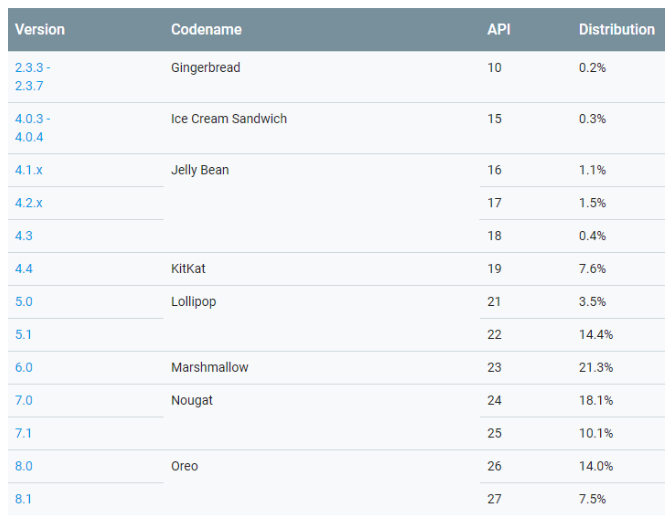
\includegraphics[width=\textwidth,height=\textheight,keepaspectratio]{mp}
		\end{center}
	\end{itemize}
\end{itemize}
\subsubsection{Cultural and Political Requirements}
\begin{itemize}
	\item CPR1: The product will not include any messages or images that will offend parties of any culture or religion.
	\begin{itemize}
		\item The application is targeted to users age 16+ (or driving age). Users should not see any offensive messages or images. If ads are present, they should be curated first to enforce this.
	\end{itemize}
	
	\item CPR2: The product will comply with current Canadian cultural standards
\end{itemize}
\subsubsection{Legal Requirements}
\begin{itemize}
	\item LR1: All assets used are either original works. It will not infringe on any copyrights and appropriate permission/licensing will be acquired.
	\item LR2: The product will comply with Canadian copyright laws.
\end{itemize}

\subsubsection{Health and Safety Requirements}
\begin{itemize}
	\item HSR1: Our application interface will pose no threat to epileptic prone users.
	
	\item HSR2: The system will provide hands-free features that will allow the user to use some functionality of the application without using their hands such as speech-to text input and text-to-speech navigation output.
	\begin{itemize}
		\item As the user is operating a motor vehicle, the system must not distract the driver to adhere to driving laws.
	\end{itemize}
\end{itemize}

\subsection{Undesired Event Handling}
In the event of a undesired event that is not a result of a previously stated assumption, the system will be designed in such a way that it will self-correct any discrepancies. This means that any desynchronization issues between the application and the servers will be fixed with the use of multiple users supplying data to the database. Additionally this will be solved by having periodic updates so that the most recent data is used. Finally, in the case of an undesired event that is not covered, the use of error handling and error messages will be utilized to prevent any confusion for the user and preventing any disastrous errors within the system. 
\section{References} 
1. Norman, D. The design of everyday things. Basic Books, New York, NY, 2013.\\
2. Google, Distribution Dashboard, Android Developers, \textit{https://developer.android.com/about/dashboards/} 2018
\end{document}
